The handling of multiple actions for the same goal would bring us closer to what
\emph{auto} or \emph{tauto} do in Coq. We could have whole theories compiled in some sort
of database and let our tool figure out which of those lemmas to apply. Since the goal is
fixed, there should be one solution. A naive extension to our library could be made:

\Agda{RW}{by+-def}

However, a \F{List} of names is a bad data structure to use here. We need to search
every single action, where, we could rule out actions purely based on their structure.
Indeed, we are going to explore an alternative data structure to speed up search and get
instantiation for free, during lookup.

\begin{TODO}
  \item cite Tries, Edward Fredkin
\end{TODO}

This section starts with a summarized explanation of Tries and then follows with our
generalization of the same concept. The structure we arrive at is a type-indexed data structure,
in the sense of \cite{Hinze04}. Yet, our lookup and insertion methods have to be significantly different
since we have to handle variables, that can be arbitralily instantiated.

\subsection{Tries}

There a few variations on of a Trie, suited for different applications. We will, however,
restrict ourselfesto the original definition, which is also the simplest. This small digression
has the purpose of introducing the underlying idea without too many technicalities.

\begin{wrapfigure}{r}{0.30\textwidth}
\begin{center}
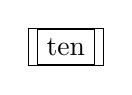
\begin{tikzpicture}[
  cnode/.style={rectangle , draw=black , fill=white},
  lbl/.style={circle , draw=none , fill=white , inner sep=0cm , font={\tiny \color{blue}}}
]
\tikzset{level 0+/.style={level distance=2cm}}
\Tree [.\node[cnode]{$\epsilon$};
        \edge node[pos=0.5 , lbl] {t};
        [.\node[cnode]{t};
           \edge node[pos=0.5 , lbl] {o};
           [.\node[cnode]{to};
             \edge[dashed] node[pos=0.5 , lbl] {tal};
             [.\node[cnode]{total}; ] 
           ]
           \edge node[pos=0.5 , lbl] {e};
           [.\node[cnode]{te};
              \edge node[pos=0.5 , lbl] {a};
              [.\node[cnode]{tea}; ]
              \edge node[pos=0.5 , lbl] {n};
              [.\node[cnode]{ten}; ]
           ] 
        ]
      ];
\end{tikzpicture}
\end{center}
\caption{Trie example}
\label{fig:firsttrie}
\end{wrapfigure}

Figure \ref{fig:firsttrie} shows a trie that stores the string set 
$S = \{ "t" , "to" , "tot" , "tota" , "total" , "te" , "tea" , "ten" \}$.
A few important notions to note are that, even though it has a tree structure, the keys are
not associated with a specific node, but with its positioning in the trie.
In the end of the day, we can look at Tries as finite deterministic acyclic automatons.

The specification of a Trie is fairly simple. Taking already a small step towards a generalization
and assuming that instead of storing lists of characters (strings) we are going to store arbitrary
lists, the Trie functor is given by:

\[
  T\;a\;k = \mu X . (k + 1) \times (a \rightarrow X + 1)
\]

So, each node contains a possible key and a partial map from $a$'s to Tries. The retrieval of
the key associated with a list $l$ is performed by recursion on $l$. When we reach the empty list
we return the $(k+1)$ part of the current node. Otherwise, we try to traverse the trie associated with the
current node partial map applied to the head of the list. 

Insertion is also very straight forward. Inserting a key $k$ indexed by a list $l$, assuming $l$ does not belong
in the trie, yet, consists of a walk in the trie, by induction $l$, adding entries to the partial maps, if needed,
until we reach the empty list, and then register $k$ at that node.

The biggest limitation of a Trie, however, is that it can only be indexed by a linear data-structure, 
such as a list. R. Hinze, J. Jeuring and A. L\"{o}h provides a solution to that, in \cite{Hinze04}, 
by defining a special kind of Tries that can be indexed by arbitrary data-types. The idea, in a nutshell,
is to work with the algebraic representation of the indexes (data-types) and have nested maps at every node.
This is a bit too general for our needs here. We are looking for a structure that can be indexed
by a given term language, which follows the tipical sum-of-products form. An additional complication
arises when we start to allow variables in the index.

\subsection{Towards a Generalization}

\begin{TODO}
  \item REWRITE!!! We specialized our Trie after all.
\end{TODO}

\newcommand{\mytrie}{NAMEIT }

Following the popular saying -- A picture is worth a thousand words -- let us begin
with a simple representation. Just like a trie, our \mytrie trie was designed to
store names of actions to be performed, indexed by their respective type. Figure 
\ref{fig:btrie1} shows the \mytrie that stores the actions from figure \ref{fig:trie1terms}.
For clarity, we have written the De Bruijn indexes of the respective variables as a superscript on
their names.

\begin{figure}[h]
\begin{eqnarray*}
  x^0 + 0 & \equiv & x^0 \\
  x^0 + y^1 & \equiv & y^1 + x^0 \\
  x^2 + (y^1 + z^0) & \equiv & (x^2 + y^1) + z^0
\end{eqnarray*}
\caption{Identity, Commutativity and Associativity for addition.}
\label{fig:trie1terms}
\end{figure}

\begin{figure}[h]
\include{img/BTrie1}
\caption{\mytrie for terms of figure \ref{fig:trie1terms}. Yellow and green circles represent DeBruijn indexes and literals, respectively.}
\label{fig:btrie1}
\end{figure}

Let us illustrate the lookup of, for instance, $(2 \times x) + 0 \equiv 2 \times x$.
The search starts by searching in the root's partial map for $\equiv$. We're given
two tries! Since $\equiv^{\star_1}$ is a binary constructor. We proceed by looking for $(2 \times x) + 0$
in the left child of $\equiv$. Well, our topmost operator is now a $+^{\star_2}$, we repeat the same idea and
now, look for $(2 \times x)$ in the left child of the left $+$. Here, we can choose
to instantiate variable 0 as $(2 \times x)$ and collect label $r_1$ or
instantiate variable 2, with the same term, and collect label $l_1$. Since we cannot know beforehand
which variable to instante, we instantiate both! At this point, the state of our lookup is
$(0 \mapsto 2 \times x , r_1) \vee (2 \mapsto 2 \times x , l_1)$.
We proceed to look for the literal $0$ in the right trie of $+^{\star_2}$, taking us to a leaf node with
a rewrite rule stating $r_1 \vdash r_2$. This reads $r_1$ should be rewritten by $r_2$. We apply
this to all states we have so far. Those that are not labeled $r_1$ are pruned. 
However, we could also instantiate variable 1 at that node, so
we add a new state $(0 \mapsto 2 \times x, 1 \mapsto 0 , k_1)$. At this step,
our state becomes $(0 \mapsto 2 \times x , r_2) \vee (0 \mapsto 2 \times x, 1 \mapsto 0 , k_1)$. 

We go up one level and find that
now, we should look for $2 \times x$ at the right child of $\equiv^{\star_1}$. We cannot traverse the
right child labeled with a $+$, leaving us with to compare the instantiation gathered for
variable 0 in the left-hand-side of $\equiv^{\star_1}$ to $2 \times x$. They are indeed the same,
which allows us to apply the rule $r_2 \vdash RI$. Which concludes the search, rewriting label $r_2$
by $RI$, or, any other code for \F{+-right-identity}. By returning not only the final label, but
also the enviroment gathered, we get the instantiation for variables for free.
The result of such search should be $(0 \mapsto 2 \times x , RI) :: []$.

This small worked example already provides a few insights not only on how to code lookup, but
also on how to define our \mytrie. We have faced two kinds of nodes. Fork nodes, which
are composed by a list of cells, and, Leaf nodes, which contain a list of (rewrite) rules.
Indeed, we define \mytrie by:

\Agda{BTrie}{btrie-rule-def}\\
\Agda{BTrie}{btrie-def}

Rewrite rules are divided in three different kinds: Gather, Transition and Final rules.
The type \F{to} comes from \texttt{\scriptsize RW.Data.PMap X IsEqX}, and represents a partial
from $X$ to some other type.

\subsection{Some notions about types}

Where $t$ is the index type and $c$ is the conclusions, or keys, we are indexing by different
elements $t_1, \cdots t_n\; :\; t$. The assumption we make, however, states that $t$ must
have a \F{IsTrie} instance. Such record is defined by:

\Agda{BTrie}{istrie-def}

Such record states that for a given $t$, there exists an index type \F{Idx}, with a decidable
underlying equality. We must be able to at least differentiate between different indexes, after all.
We also state the we must be able to open and close such term. It is easy to prove that for each
sum-of-products recursive type, we can construct a type \F{Idx} satisfying these properties.
Just ignore the recursive arguments and make a label for each constructor.

The indexes for \D{RTerm} datatype are defined by:

\Agda{BTrie}{rterm-idx-data}

One interesting part, however, is the \F{toSym} function. These \F{Sym}bols are the binding
symbols. We are stating that some of our indexes are in fact binding symbols, therefore
we need a way to both distinguish between binding and non-binding indexes, and convert
to a standard representation. DeBruijn indexes were adopted as this representation.

\subsection{Lookup}

\begin{TODO}
  \item Explain my lookup monad.
  \item Present the algorithm.... which language?
\end{TODO}

\subsection{Insertion}
